% !TEX TS-program = xelatex
% !BIB TS-program = bibtex
\documentclass[12pt,letterpaper]{article}
\usepackage{style/dsc180reportstyle}
\usepackage{colortbl}
\definecolor{acchi}{HTML}{C8E6C9}
\definecolor{accmid}{HTML}{FFF9C4}
\definecolor{acclo}{HTML}{FFCDD2}
\newcommand{\tightlegendbox}[2]{\begingroup\setlength{\fboxsep}{1pt}\colorbox{#1}{#2}\endgroup}

\newcommand{\BaseMean}{62.4}
\newcommand{\BaseStd}{10.8}
\newcommand{\BaseMin}{40.0}
\newcommand{\BaseMax}{80.0}
\newcommand{\MargMean}{64.5}
\newcommand{\MargStd}{11.8}
\newcommand{\MargMin}{35.3}
\newcommand{\MargMax}{83.3}
\newcommand{\VoteMean}{56.1}
\newcommand{\VoteStd}{11.1}
\newcommand{\VoteMin}{30.0}
\newcommand{\VoteMax}{77.5}
\newcommand{\TemporalFirstTime}{2.5s}
\newcommand{\TemporalPeakAcc}{61.0}
\newcommand{\TemporalPeakTime}{25.0}
\newcommand{\TemporalFinalAcc}{53.0}
\newcommand{\TemporalFinalTime}{57.5}
\newcommand{\FamAllAcc}{56.8}
\newcommand{\FamHighAcc}{71.2}
\newcommand{\FamLowAcc}{65.7}
\newcommand{\FamHighN}{28}
\newcommand{\FamLowN}{29}
\newcommand{\LikeCount}{638}
\newcommand{\DislikeCount}{642}
\newcommand{\LikePct}{49.8}
\newcommand{\DislikePct}{50.2}
\newcommand{\SoneMarginN}{27}
\newcommand{\SoneMarginRemoved}{32}


\title{Decoding music preference from EEG}

\author{Jason Tran \\
  {\tt jat037@ucsd.edu} \\[4pt]
  COGS 189: Brain-Computer Interfaces \\
  University of California San Diego}

\begin{document}
\maketitle

\begin{abstract}
This project investigates whether binary music preference (like versus dislike) can be decoded
from electroencephalography (EEG) recorded while participants listened to one-minute music video
excerpts. Using the DEAP dataset (32 subjects, 40 trials each), we extract a 164-dimensional
feature set combining differential entropy across five frequency bands with frontal alpha
asymmetry (FAA), and evaluate three classification strategies under 5-fold stratified
cross-validation. The best strategy achieves a mean within-subject accuracy of \MargMean\%
using margin-based label binarization. SHAP analysis reveals that all four FAA features occupy
the top four positions globally, providing strong support for the approach-withdrawal
hypothesis. Time-resolved decoding shows preference information is first decodable within
\TemporalFirstTime{} and peaks at \TemporalPeakAcc\% near \TemporalPeakTime{} seconds.
Both high- and low-familiarity conditions exceed the overall baseline, with high-familiarity
trials reaching \FamHighAcc\%.
\end{abstract}

\clearpage
\maketoc
\clearpage

% =============================================================================
\section{Introduction \& background}

Music preference is a subjective phenomenon with measurable correlates in neural activity.
When a person hears music they enjoy, changes in cortical activity appear within seconds,
particularly in frontal regions associated with reward and approach motivation. Decoding these
preferences directly from EEG signals would have applications in passive music recommendation
and the neuroscience of aesthetic experience.

The theoretical backbone of this work is the approach-withdrawal model of
\citet{davidson1992anterior}, which claims that preferred stimuli are associated with greater
left frontal cortical activation, while disliked stimuli engage the right hemisphere. In EEG,
this asymmetry is visible in the alpha band (8--13 Hz) through the frontal alpha asymmetry
(FAA) index:
\[
  \mathrm{FAA} = \ln(\alpha_{\mathrm{right}}) - \ln(\alpha_{\mathrm{left}}).
\]
A positive FAA value indicates greater left frontal activation. We hypothesize that FAA
features will rank among the most predictive of the feature set.

Our pipeline consists of four stages: (1) data exploration and binarization of the continuous
liking scale, (2) feature engineering, (3) within-subject
cross-validated classification, and (4) model interpretability.

% =============================================================================
\section{Data \& features}

\subsection{Dataset}

The DEAP dataset \citep{koelstra2012deap} contains physiological recordings from 32
participants (16 male, 16 female; ages 19--37) while they watched 40 one-minute music video
excerpts. After each excerpt, participants rated their emotional response on four 9-point
continuous scales: valence (unhappy to happy), arousal (calm to excited), dominance
(submissive to in-control), and liking (dislike to like). Only the liking dimension is used
as the target variable.\footnote{EEG was recorded with a 32-channel BioSemi ActiveTwo cap following
the 10--20 system at 512 Hz, then downsampled to 128 Hz. Each trial consists of a 3-second
baseline epoch followed by a 60-second stimulus epoch, yielding 7,680 samples per trial and
1,280 trials in total.}

Table~\ref{tab:ratings} summarizes descriptive statistics for all four dimensions across all
1,280 trials. We binarize continuous liking scores via a median split per-subject, yielding a
near-balanced class distribution (\LikeCount{} like, \DislikeCount{} dislike). A second
strategy, margin binarization, removes trials within $\pm 0.5$ rating units of the median to
exclude ambiguous labels at the cost of reduced sample size (e.g., subject 1 retains
\SoneMarginN{} of 40 trials, removing \SoneMarginRemoved\%).

\begin{table}[H]
  \centering
  \caption{Descriptive statistics of self-report ratings across all subjects and trials ($n = 1{,}280$).}
  \label{tab:ratings}
  \begin{tabular}{lrrrrr}
    \toprule
    Dimension & Mean & Std & Min & Max & Median \\
    \midrule
    Valence & 5.25 & 2.13 & 1.0 & 9.0 & 5.04 \\
    Arousal & 5.16 & 2.02 & 1.0 & 9.0 & 5.23 \\
    Dominance & 5.38 & 2.10 & 1.0 & 9.0 & 5.24 \\
    Liking & 5.52 & 2.28 & 1.0 & 9.0 & 6.05 \\
    \bottomrule
  \end{tabular}
\end{table}


\begin{figure}[H]
  \centering
  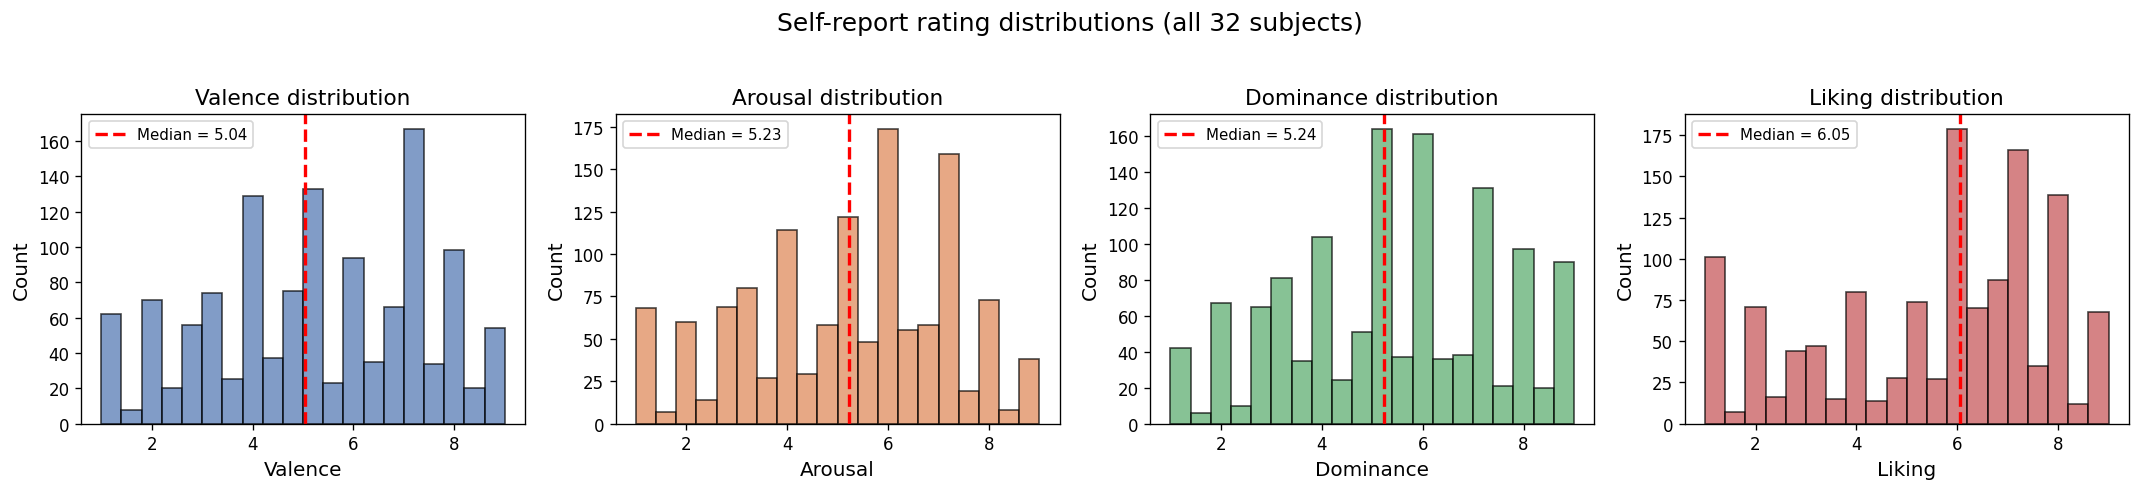
\includegraphics[width=\linewidth]{report_files/report_8_1.png}
  \caption{Distributions of self-report ratings across all 1,280 trials. All four dimensions
    span the full 1--9 range.}
\end{figure}

The 32 electrodes span frontal, central, parietal, occipital, and temporal regions
(Figure~\ref{fig:electrodes}). Frontal coverage is particularly important for FAA, which
relies on paired symmetric electrodes. Figure~\ref{fig:psd} shows a representative power
spectrum.

\begin{figure}[H]
  \centering
  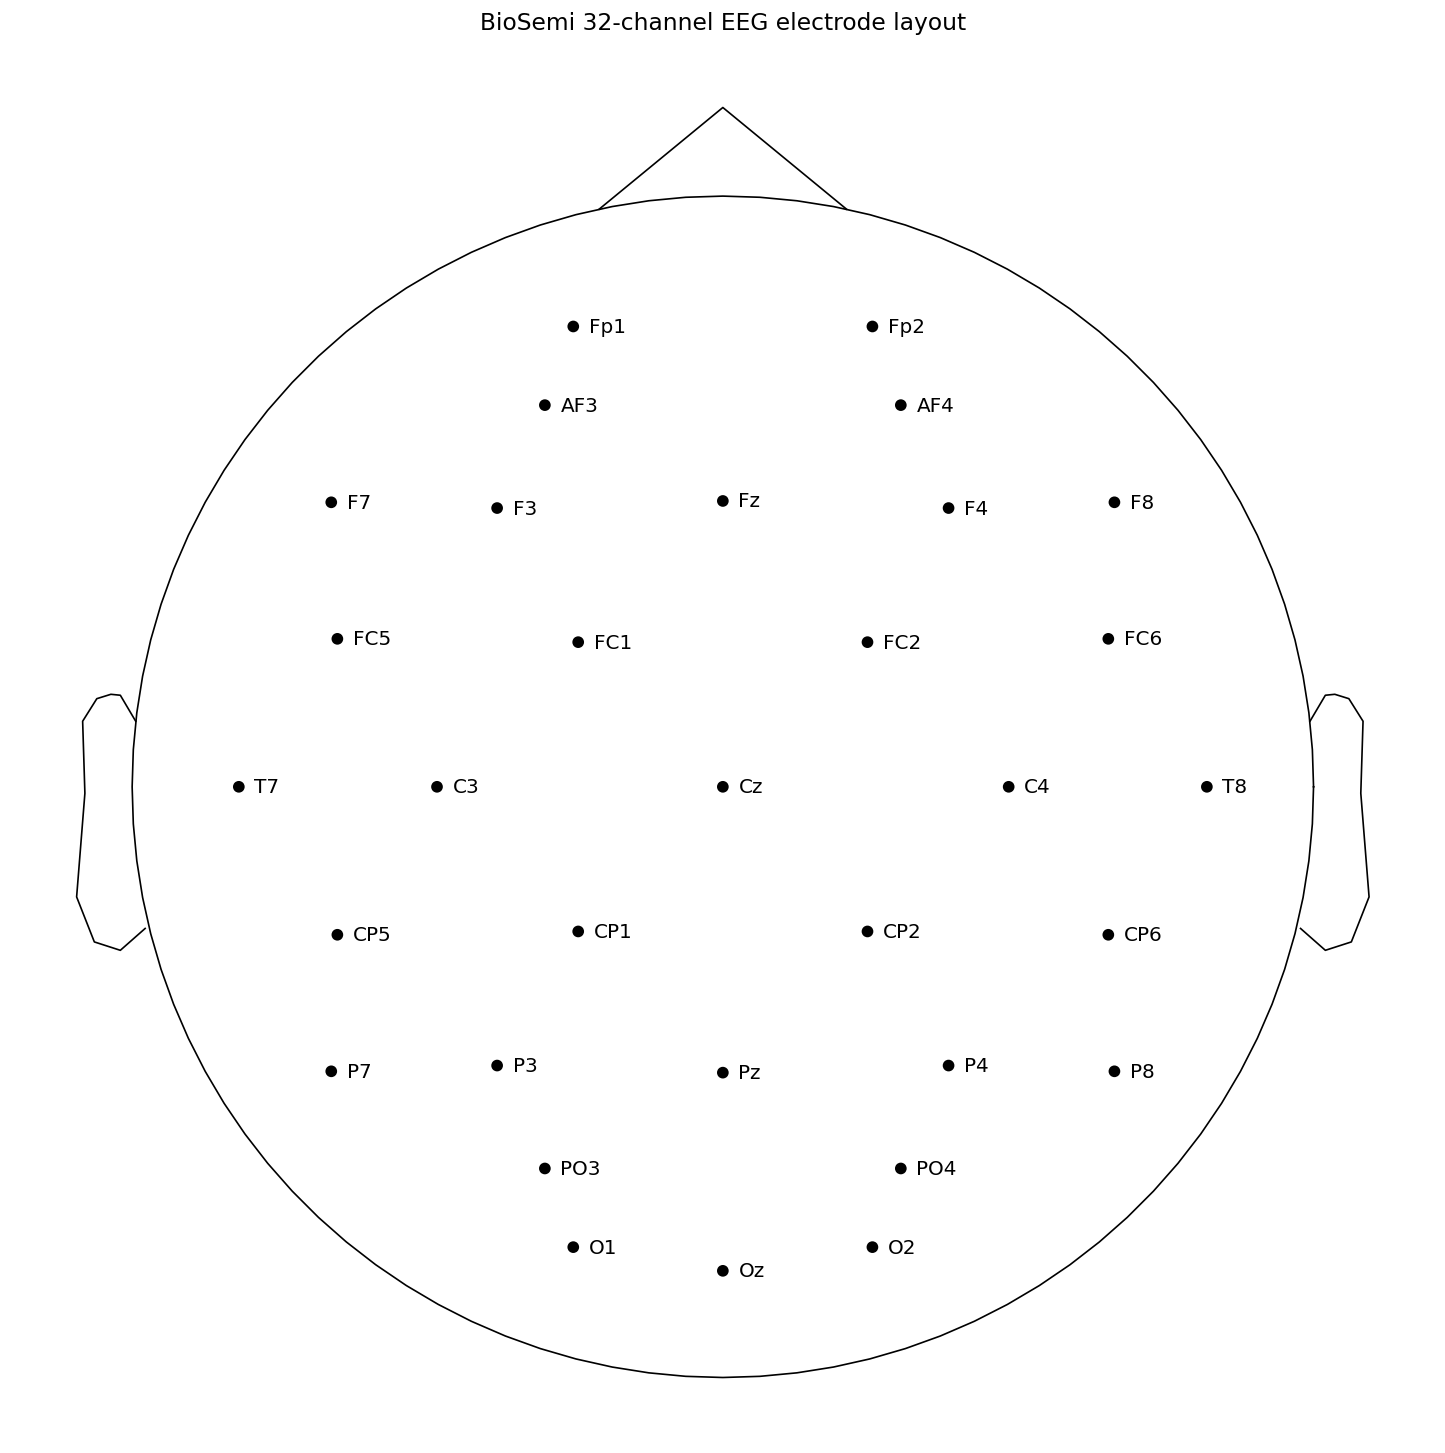
\includegraphics[width=0.5\linewidth]{report_files/report_12_0.png}
  \caption{BioSemi 32-channel electrode layout. Frontal pairs used for FAA are Fp2/Fp1,
    AF4/AF3, F4/F3, and F8/F7.}
  \label{fig:electrodes}
\end{figure}

\begin{figure}[H]
  \centering
  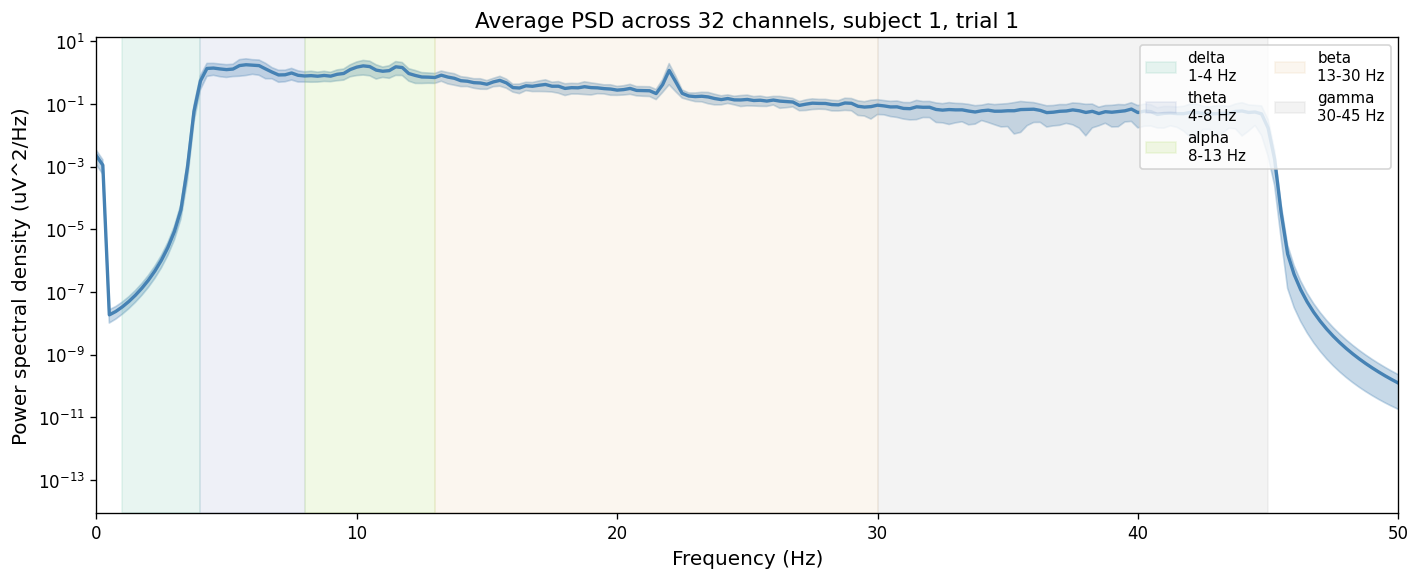
\includegraphics[width=\linewidth]{report_files/report_14_1.png}
  \caption{Mean power spectral density averaged across all channels for subject 1, trial 1.}
  \label{fig:psd}
\end{figure}

\subsection{Feature engineering}

Differential entropy (DE) quantifies the information content of a continuous signal. Under
the assumption of a Gaussian distribution, it reduces to:
\[
  \mathrm{DE}(x) = \tfrac{1}{2} \ln(2 \pi e \, \sigma^2),
\]
where $\sigma^2$ is the band-limited power estimated via Welch's method. DE is computed for
each of the 32 channels across five frequency bands (delta 1--4 Hz, theta 4--8 Hz, alpha
8--13 Hz, beta 13--30 Hz, gamma 30--45 Hz), yielding a 160-dimensional feature vector. DE
has been shown to outperform raw band power for EEG-based emotion recognition
\citep{duan2013differential}. Figure~\ref{fig:de} shows a representative DE heatmap.

The FAA index is computed for four symmetric frontal electrode pairs (Fp2/Fp1, AF4/AF3,
F4/F3, F8/F7), each contributing one feature. Figure~\ref{fig:faa} shows the distribution of
FAA values by preference label. Combined with DE, the full feature vector has 164 dimensions.

\begin{figure}[H]
  \centering
  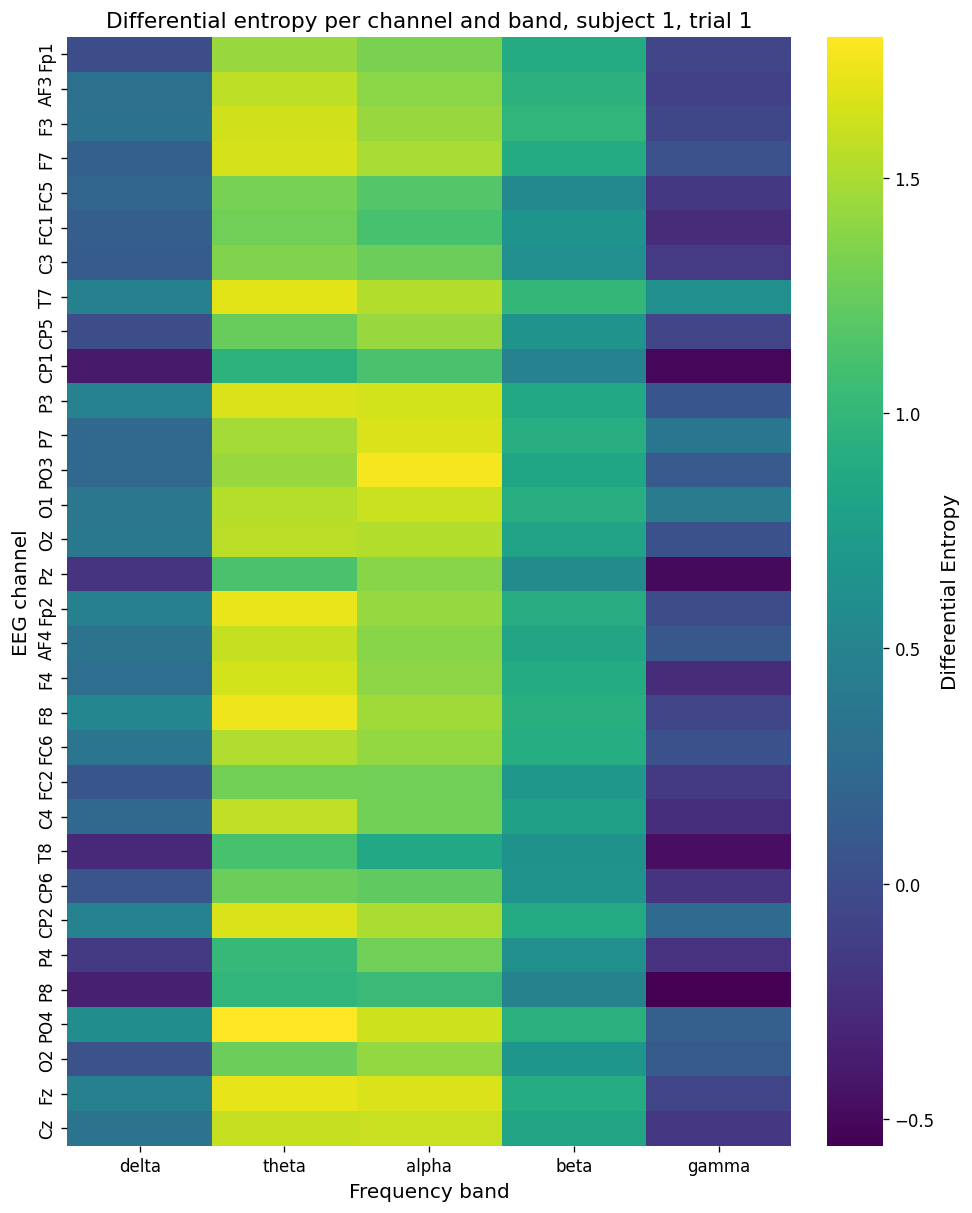
\includegraphics[width=\linewidth]{report_files/report_16_1.png}
  \caption{Differential entropy heatmap for subject 1, trial 1.}
  \label{fig:de}
\end{figure}

\begin{figure}[H]
  \centering
  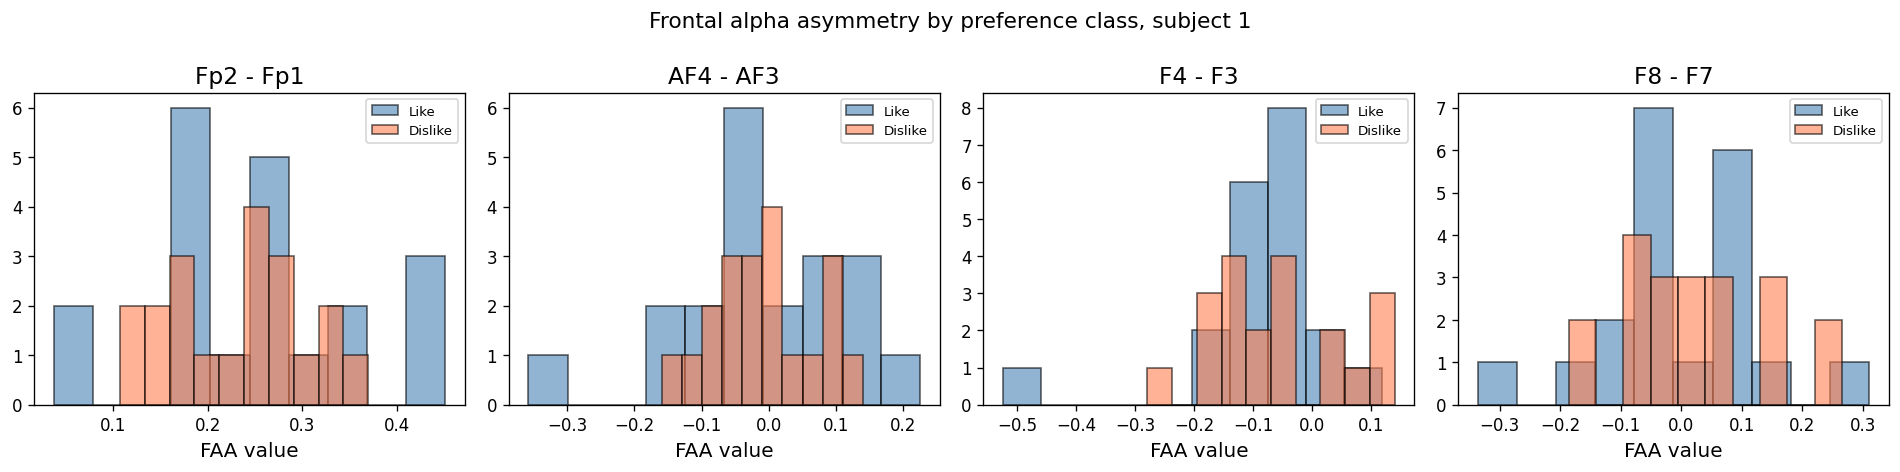
\includegraphics[width=\linewidth]{report_files/report_18_2.png}
  \caption{Distribution of FAA values for each frontal pair, split by binary preference label.
    Positive FAA indicates greater left frontal activation.}
  \label{fig:faa}
\end{figure}

% =============================================================================
\section{Classification}

\subsection{Methods}

All classifiers are evaluated under 5-fold stratified cross-validation within each subject.
Three strategies are compared:

\begin{enumerate}{}
  \item Baseline: 164-dimensional features with median-split binarization. Three classifiers
    are trained independently (SVM with RBF kernel, XGBoost, and random forest), and the best
    per-subject result is reported.
  \item Baseline with margin binarization: we do the same as above, but trials within $\pm 0.5$ rating
    units of the per-subject median are removed.
  \item Majority-vote ensemble: XGBoost, random forest, and LightGBM combined by majority
    vote, after variance filtering and mutual-information feature selection retaining 50
    features.
\end{enumerate}

\subsection{Results}

Margin binarization improves mean accuracy from \BaseMean\% to \MargMean\%
(Table~\ref{tab:results}), confirming that removing ambiguous trials results in cleaner class
boundaries. The majority-vote ensemble underperforms the single-model baseline (\VoteMean\%),
likely because aggressive feature selection discards information. Inter-subject
variability is substantial (range \MargMin--\MargMax\%), reflecting the highly individual
nature of preference-related neural representations (Figure~\ref{fig:persubject}).
Table~\ref{tab:persubject} reports individual results; several subjects fall at or below
chance, indicating that the feature set is not a catch-all for all individuals.

\input{data/table_aggregate}

\begin{figure}[H]
  \centering
  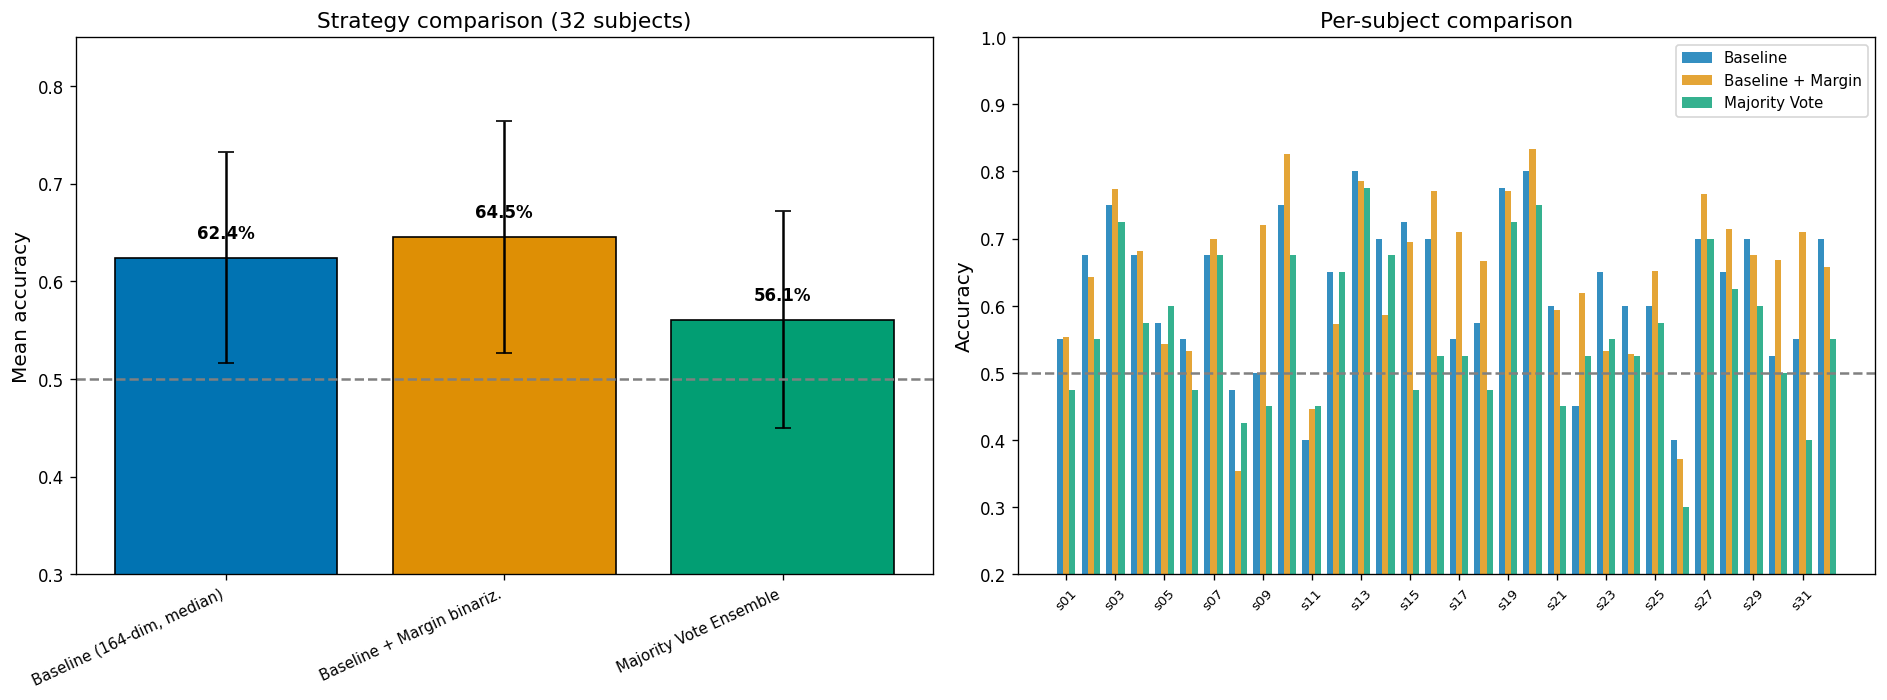
\includegraphics[width=\linewidth]{report_files/report_28_1.png}
  \caption{Per-subject accuracy for the three classification strategies.}
  \label{fig:persubject}
\end{figure}

\input{data/table_persubject}

% =============================================================================
\section{Interpretability \& advanced analysis}

\subsection{SHAP feature importance}

SHAP (SHapley Additive exPlanations) values were computed using a \texttt{TreeExplainer}
\citep{lundberg2017unified} on XGBoost models trained for each of the 32 subjects. Feature
importance is estimated as the mean absolute SHAP value per feature, averaged across subjects.

\begin{figure}[H]
  \centering
  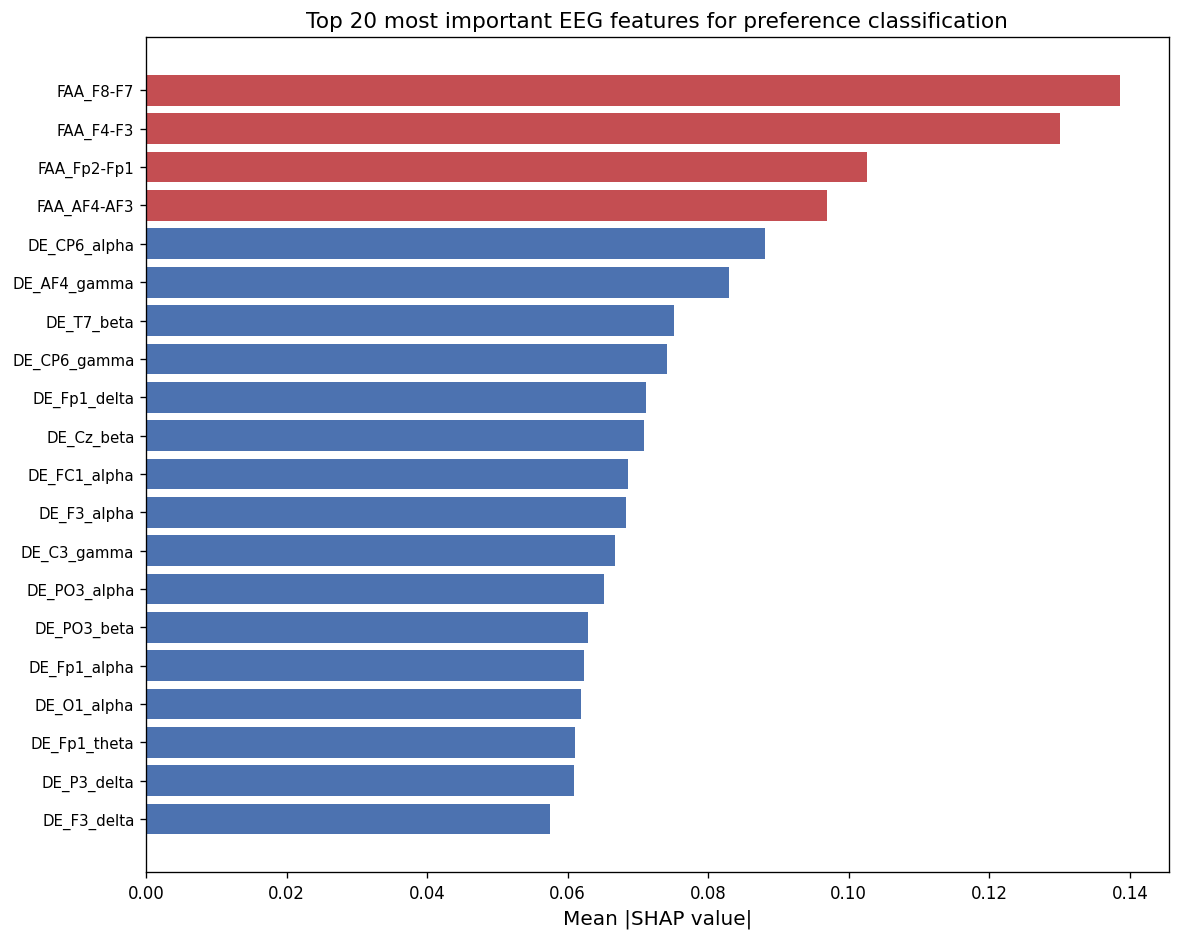
\includegraphics[width=\linewidth]{report_files/report_32_1.png}
  \caption{Top 20 features by mean absolute SHAP value, averaged across all 32 subjects.}
\end{figure}

Strikingly, all four FAA features occupy the top four positions in global importance
(Table~\ref{tab:shap}), with FAA at the F8--F7 pair ranking first. This constitutes strong
support for the approach-withdrawal hypothesis, as frontal alpha asymmetry is not merely present
but is the dominant class of predictor. The remaining top features are DE features spanning
alpha, gamma, beta, and delta bands, concentrated at frontal, parietal, and temporal
electrodes.

\input{data/table_shap}

\begin{figure}[H]
  \centering
  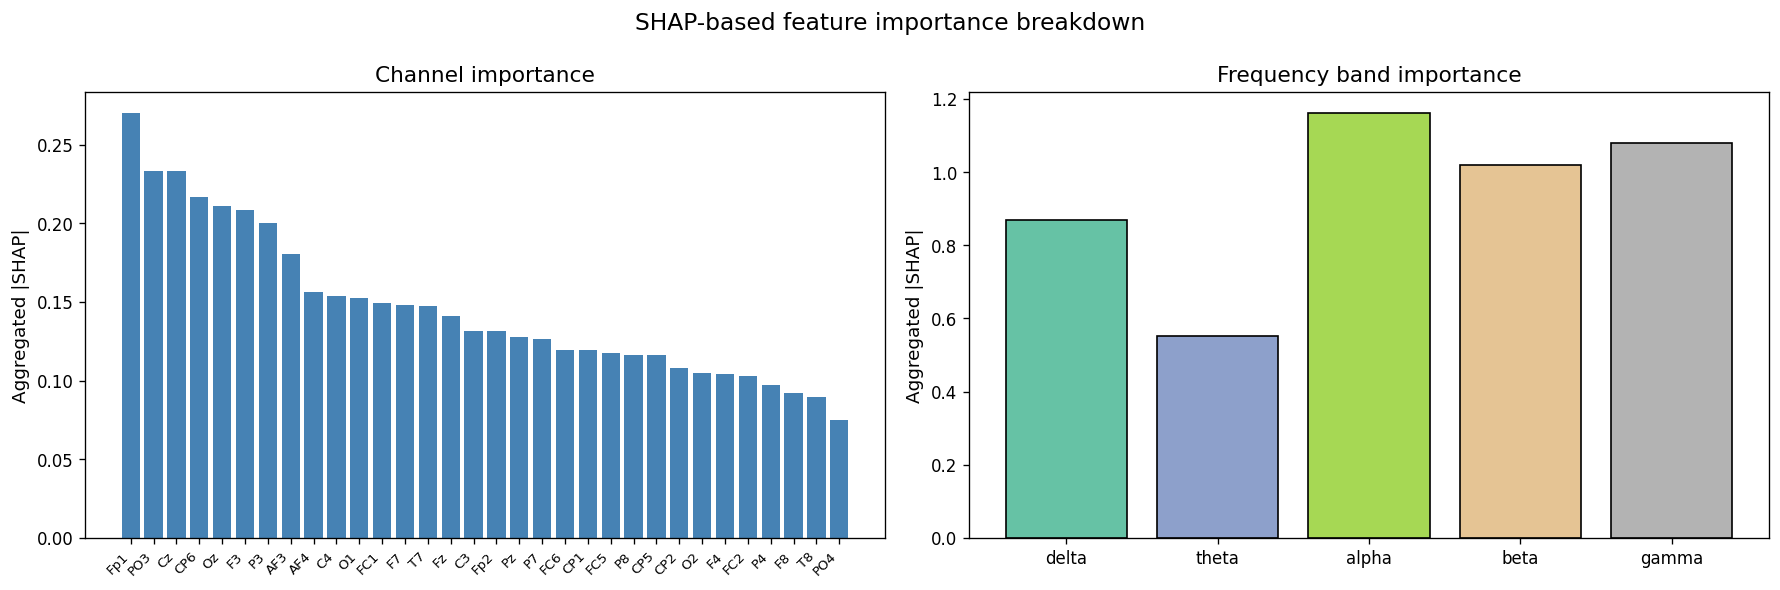
\includegraphics[width=\linewidth]{report_files/report_34_1.png}
  \caption{Aggregated SHAP importance by channel (left) and frequency band (right).}
\end{figure}

\begin{figure}[H]
  \centering
  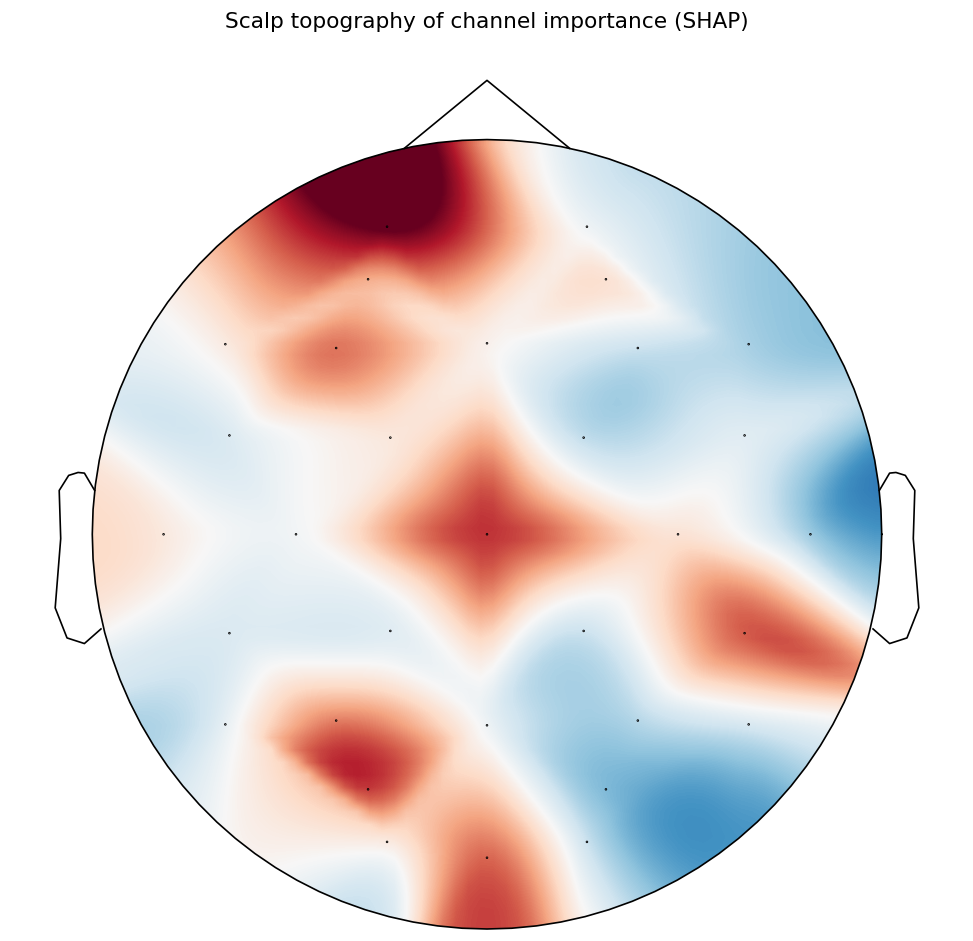
\includegraphics[width=0.55\linewidth]{report_files/report_36_0.png}
  \caption{Scalp topographic map of channel-level SHAP importance summed across all frequency
    bands.}
\end{figure}

\subsection{Time-resolved decoding}

To identify when during a trial preference information becomes decodable, features were
extracted from 5-second sliding windows with a 2.5-second step across the full 60-second
trial for five representative subjects (s01, s03, s05, s08, s16).

\begin{figure}[H]
  \centering
  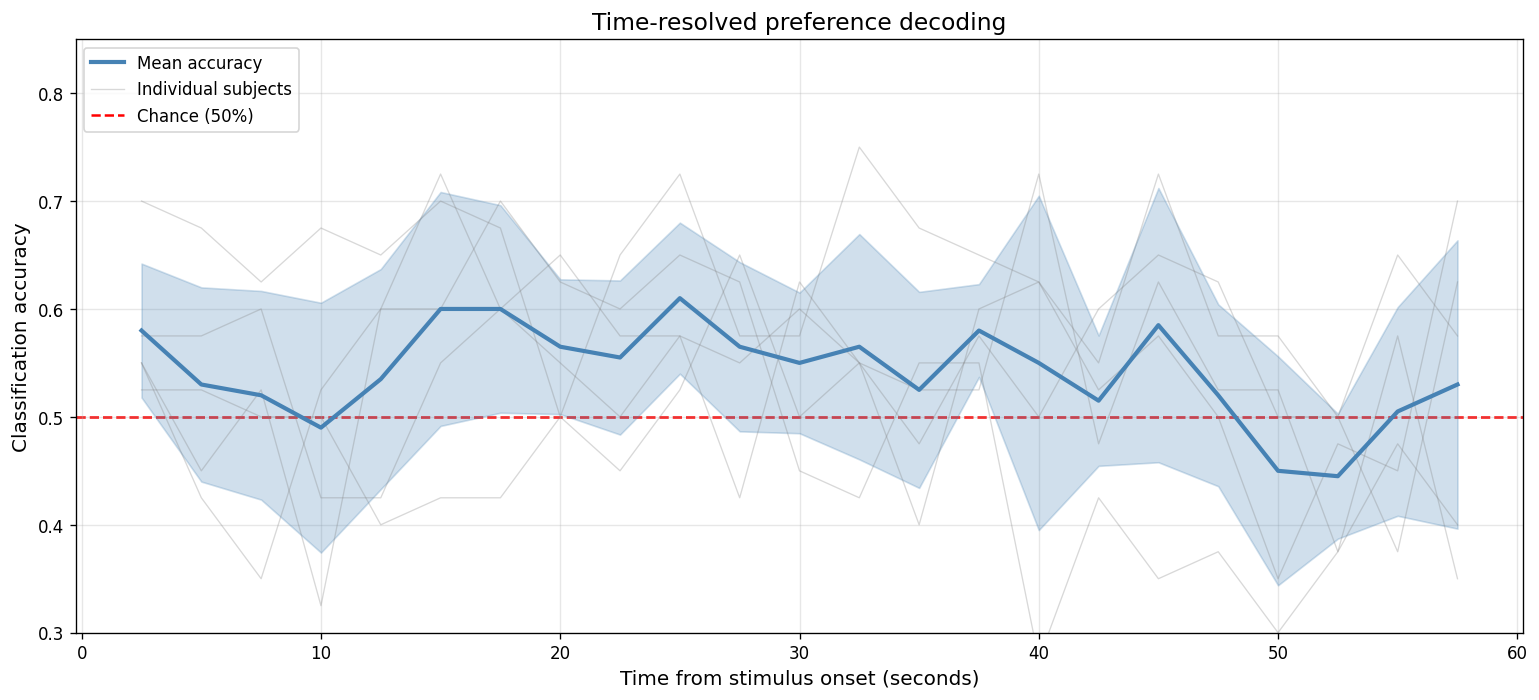
\includegraphics[width=\linewidth]{report_files/report_39_1.png}
  \caption{Time-resolved decoding accuracy for five representative subjects. Shading shows
    $\pm 1$ standard error across folds.}
\end{figure}

Decoding first exceeds the 55\% threshold at approximately \TemporalFirstTime{} after trial
onset. Peak group accuracy is \TemporalPeakAcc\% at \TemporalPeakTime{} seconds, after which
accuracy declines, stabilizing at \TemporalFinalAcc\% at \TemporalFinalTime{} seconds. The
early onset suggests evaluation is rapidly effective, while the mid-trial peak and subsequent
decline may reflect loss of or shifting attention over the course of the video clip.

\subsection{Familiarity disentanglement}

Song familiarity is a reasonable confound, since prior exposure to a track may strengthen
preference-related neural signals independently of the current listening experience. Trials
were split by familiarity rating into high- and low-familiarity subsets, and classification
was repeated for all 32 subjects.

\begin{figure}[H]
  \centering
  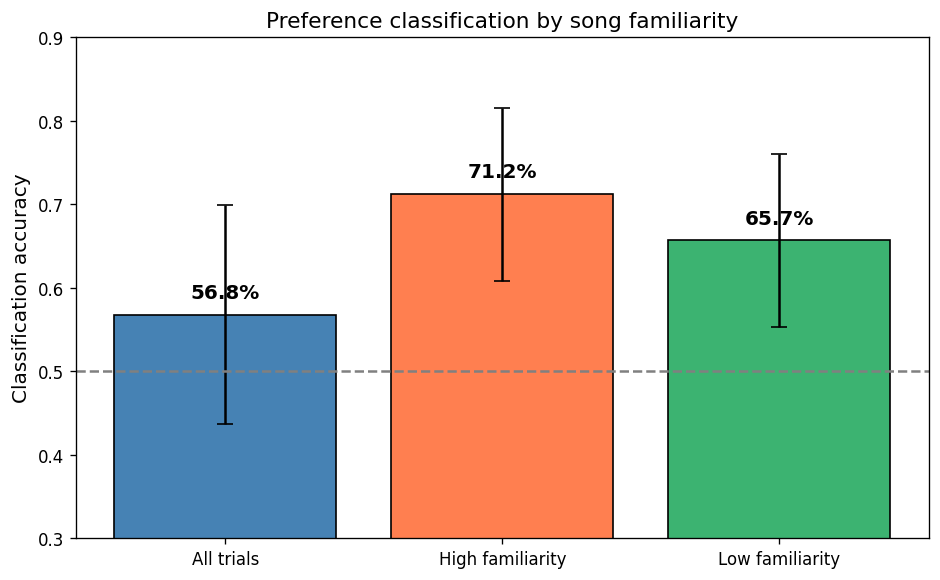
\includegraphics[width=0.7\linewidth]{report_files/report_43_1.png}
  \caption{Classification accuracy under three familiarity conditions.}
\end{figure}

\begin{table}[H]
  \centering
  \caption{Familiarity disentanglement results.}
  \label{tab:familiarity}
  \begin{tabular}{lccc}
    \toprule
    Condition & Mean accuracy (\%) & Std (\%) & $n$ subjects \\
    \midrule
    All trials & 56.8 & 13.2 & 32 \\
    High familiarity only & 71.2 & 10.3 & 28 \\
    Low familiarity only & 65.7 & 10.4 & 29 \\
    \bottomrule
  \end{tabular}
\end{table}


Both familiarity conditions substantially exceed the all-trials baseline (\FamAllAcc\%),
suggesting that when the analysis is restricted to trials with clear familiarity status,
classification improves markedly. The high-familiarity advantage over low-familiarity
(\FamHighAcc\% versus \FamLowAcc\%) is consistent with the hypothesis that prior exposure
consolidates preference-related neural representations.

% =============================================================================
\section{Discussion \& summary}

Binary music preference is decodable from EEG at above-chance accuracy when we are
principled and intentional with our feature engineering. The best mean accuracy of \MargMean\% is achieved with margin
binarization, compared to a 50\% chance baseline, with individual subjects ranging from
\MargMin\% to \MargMax\%.

The most striking finding is that all four FAA features occupy the top four positions in
global SHAP importance, which constitutes strong support for the approach-withdrawal hypothesis.
Frontal alpha asymmetry is not merely present but is the dominant class of predictor.

Preference information is decodable within the first \TemporalFirstTime{} and peaks near
\TemporalPeakTime{} seconds (\TemporalPeakAcc\%), after which accuracy declines toward
\TemporalFinalAcc\% at trial end. The familiarity analysis shows that both high- and
low-familiarity conditions improve over the all-trials baseline (\FamHighAcc\% and
\FamLowAcc\% versus \FamAllAcc\%).

% =============================================================================
\makereference
\bibliography{reference}
\bibliographystyle{style/dsc180bibstyle}

\end{document}
